\documentclass[a4paper,11pt]{report}
\usepackage{graphicx}
\usepackage{float}
\usepackage{subfig}
\usepackage{geometry}
\usepackage{amsmath,amssymb}
\usepackage{amsthm}
\usepackage{bbold}
\usepackage{mathtools}
\usepackage{braket}
\usepackage{booktabs}
\usepackage[table,xcdraw]{xcolor}
\usepackage[utf8]{inputenc}
\usepackage{cite}
\usepackage[english]{babel}
\usepackage{lipsum}
\usepackage{setspace}
\usepackage{minted}
\usepackage{xcolor}
\usepackage{hyperref}
\hypersetup{colorlinks=true,linkcolor=blue}
\geometry{a4paper, top=2.5cm, bottom=2.5cm, left=3cm, right=2.5cm}

\begin{document}
	
\section*{Problem 1}
In the first problem it is required to write a function that computes the LU factorization of a non-singular matrix $A$ without pivoting. The full code has been written using Python as programming language and it is available at the following link on GitHub **** INSERIRE LINK ****, where it is also possible to find a link to the online documentation **** INSERIRE LINK **** \footnote{The syntax used in the docstrings of the Python functions is necessary to obtain clear latex formatting of the formulas in the online documentation.}.\\
In the following it is reported the function \mintinline{python}{lufact(A)} that can be found in the library named Project\_1.py

\begin{minted}[mathescape, linenos, gobble=0, breaklines]{python}
def lufact(A):
 r''' This function computes the LU factorization of a non-singular matrix A without pivoting, giving as output the matrices L and U and the growth factor g, here defined as :math:`\frac{max_{ij} (|L||U|)_{ij}}{max_{ij} (|A|)_{ij}}`.

 Paramters:
 ----------
 A : ndarray
     input matrix of dimension :math:`(N\times N)`
	
 Returns
 -------
 L : ndarray
     Unit lower triagular matrix
 U : ndarray
     Upper triangular matrix
 g : ndarray
     growth factor
 '''

 # Compute the dimension of the input square matrix
 dim = A.shape
 n = dim[0]

 # Define the chosen precision
 precision = np.finfo(float).eps

 # Check that the input matrix is a square matrix
 assert (dim[0] == dim[1]), "The input matrix is not a square matrix"

 # Check if the input matrix is singular
 if np.abs(np.linalg.det(A)) < precision:
    logging.warning("The input matrix is singular")
 # Check if the hypothesis of the LU factorization theorem hold
 for k in range(n):
    if np.abs(np.linalg.det(A[:k+1,:k+1])) < precision:
	   logging.warning(f'The {k}-th principal minor is less than the chosen precision')

 # Create a copy of the input matrix to be modified in order to obatin the matrices L and U
 B = np.copy(A)
 for k in range(0,n-1):
   for i in range(k+1,n):
      B_kk = B[k,k]
      # Check if there is a division by a quantity smaller than the chosen precision
      if np.abs(B_kk) < precision:
         raise ValueError('Division by a quantity smaller than the chosen precision - B_kk = {B_kk}')
      B[i,k] = B[i,k]/B_kk
   for j in range(k+1,n):
      for l in range(k+1,n):
         B[l,j] = B[l,j] - B[l,k]*B[k,j]

 # Extract the matrices L and U from B using, resepctively, a strictly lower triangular mask and an upper triangular mask.
 L = np.tril(B,k=-1) + np.eye(n) # Add the Id matrix in order for L to be unit lower triangular
 U = np.triu(B,k=0)  

 # Compute the growth factor
 LU_abs = np.abs(L)@ np.abs(U)
 g = np.amax(LU_abs)/np.amax(np.abs(A))

 return L, U, g
\end{minted}

\noindent We included tests in this function in order to ensure that the input matrix has the correct characteristics to perform the LU factorization. The rationale used to insert such tests is explained in the following. We added \textit{warnings}, using the \mintinline{python}{logging} Python library, for all the checks that, if not satisfied, do not necessarily break the LU factorization, so the flow of the code does not interrupt. We expect these to be some of the cases where the LU factorization gives higher errors in terms of relative backward stability *** NON SONO SICRA CHE SIA VERAMENTE COSI' ***
For what concern most significant errors, we inserted an \textit{assertion} if the input matrix is not square (even if it is clarified in the function's docstring that it must be square), so that the flow of the code is interrupted, and a \textit{ValueError} if a division by a quantity smaller than the chosen precision occurs. In this last case, if the LU factorization fails, this information is stored in a counter in the main program (see subsection \ref{subsect:Main_Program}) and it is saved in an Excel file for all the types of matrices and the dimensions considered. The counter will be updated each time a failure occurs.\\

\noindent In analyzing the results regarding the correctness of the computational LU factorization for the chosen input matrices, it is required to study the trend of the growth factor and the relative backward error with respect to the dimension of the considered matrices. While the growth factor is computed within the function \mintinline{python}{lufact(A)}, the relative backward error must be computed separately. The code that computes this value is reported below.

\begin{minted}[mathescape, linenos, breaklines]{python}
def relative_backward_error(A,L,U):
 r''' This function computes the relative backward error of the LU factorization, defined as :math:`\frac{\lVert A -LU \rVert_{\infty}}{\lVert A \rVert_{\infty}}`

 Parameters
 ----------
 A : ndarray
     Input matrix
 L : ndarray
     Unit lower triangular matrix, obtained from the LU factorization of the input matrix A.
 U : ndarray
     Upper triangular matrix, obtained from the LU factorization of the input matrix A.

 Returns
 -------
 out : float
       Relative backward error
'''

 return np.linalg.norm(A - L @ U, ord=np.inf)/np.linalg.norm(A, ord=np.inf)
\end{minted}

\noindent Note that the symbol \mintinline{python}{@} stands for the operator that performs the matrix multiplication.\\

\noindent Once having constructed these functions, we built the dataset of matrices, on which apply the LU factorization, by creating a function that takes two values as input, namely the number of matrices of each type and their dimension, and gives as output a dictionary containing all the sampled matrices of each type. In particular, we considered random matrices, unitary matrices, Hermitian matrices, positive definite matrices and diagonally dominant matrices. For the fist type of matrices, we distinguished matrices whose entries are real and uniformly sampled in the range $\left[0,1\right)$ and matrices whose entries are independent complex and normally distributed. Secondly, to sample unitary and Hermitian matrices we considered, instead, ensembles of random matrices using the \mintinline{python}{tenpy} library in Python. Moreover, positive definite matrices are sampled using the \mintinline{python}{qutip} library in Python, by considering trace-one matrices of the form $A^{*}A$, where $A^{*}$ stands for the Hermitian conjugate of the matrix $A$, sampled as a matrix whose entries are independent complex and normally distributed. Finally, we define a function to sample diagonally dominant matrices, which is reported below.\\

\noindent In this last case the idea is to generate random matrices whose entries are normally distributed and substitute the diagonal element with a new one obtained by summing the absolute values of all the elements in the corresponding row (including itself). The sign of the diagonal element is chosen at random, by generating $N$ numbers in the interval $\left[0,1\right)$ and applying the sign function to these numbers, shifted by $0.5$.

\begin{minted}[mathescape, linenos, breaklines]{python}
def diagonally_dominant_matrix(N):
 ''' This function returns a diagonally dominant matrix of dimension :math:`(N\times N)`, whose non-diagonal entries are normally distributed.

 Parameters
 ----------
 N : int
 Dimension of the output matrix

 Returns
 -------
 out : ndarray
 Diagonally dominant matrix

 '''
 # The following steps are made to decide the sign of the diagonal element of the output matrix
 # Obtain N random numbers in [0,1) and apply the sign function to this values, shifted by 0.5
 diag_sign = np.random.rand(N)
 diag_sign = np.sign(diag_sign - 0.5)
 diag_sign[diag_sign == 0] = 1 # Set to 1 the (vary improbable) values equal to 0

 # Obtain a matrix of dimension (NxN) whose entries are normally distributed
 M = np.random.normal(loc=0.0, scale=1.0, size=(N,N))
 # Substitute all the diagonal elements in this matrix with the sum of the absolute values of all the elements in the corresponding row (including itself)
 for i in range(N):
    M[i,i] = sum(np.abs(M[i,:])) * diag_sign[i]

 return M
\end{minted}

\noindent The function that creates the dataset of matrices is reported in the following. Note that we have fixed the seed to have reproducibility of the results (\mintinline{Python}{tenpy} and \mintinline{Python}{qutip} libraries work using \mintinline{Python}{numpy} in the background, so this choice for the seed holds for all the sampled matrices). We have decided to use dictionaries to define the result of this function in order to have a better control the flow of the code in the main program and ensure an easily readability of the input data.
\begin{minted}[mathescape, linenos, breaklines]{python}
def create_dataset(num_matr,dim_matr):
 ''' This function creates the dataset, taking as input the number of matrices of each type and their relative dimension and giving as output a dictionary whose keys represent the different types of matrices considered and whose values are 3-dimensional arrays, where the first index cycles on the number of matrices considered. The output matrices are chosen to be nonsingular.

 Parameters
 ----------
 num_matr : int
            Number of matrices for each type
 dim matr : int
            Dimension of the (square) matrices

 Returns
 -------
 out : dictionary
       Dictionary whose keys represent the different types of matrices considered. Each value of the dictionary is an array of shape (num_matr,dim_matr,dim_matr).
'''

 # Define the minimum value of the determinant of the dataset matrices
 precision_zero = np.finfo(float).tiny

 # Set the seeds to have reproducibility of the results
 np.random.seed(1)

 # Create arrays to store the final matrices
 Random = np.zeros((num_matr,dim_matr,dim_matr))
 Ginibre = np.zeros((num_matr,dim_matr,dim_matr), dtype=complex)
 CUE = np.zeros((num_matr,dim_matr,dim_matr), dtype=complex)
 GUE = np.zeros((num_matr,dim_matr,dim_matr), dtype=complex)
 Wishart = np.zeros((num_matr,dim_matr,dim_matr), dtype=complex)
 Diag_dom = np.zeros((num_matr,dim_matr,dim_matr))

 # Define a dictionary to keep track of the types of matrices chosen
 dataset = {'Random':Random, 'Ginibre':Ginibre, 'CUE':CUE, 'GUE':GUE, 'Wishart':Wishart, 'Diagonally dominant':Diag_dom}

 # Random matrices: matrices whose entries are in [0,1)
 i = 0
 while i < num_matr:  
  matrix = np.random.rand(dim_matr,dim_matr)
  if np.abs(np.linalg.det(matrix)) < precision_zero:
     pass
  else:
     dataset['Random'][i,:,:] = matrix
  i = i + 1
 logging.info('Random matrices generated')

 # Ginibre matrices: matrices whose entries are independent, complex, and normally distributed
 i = 0
 while i < num_matr:  
  matrix = np.random.normal(loc=0.0, scale=1.0, size=(dim_matr,dim_matr)) + 1j*np.random.normal(loc=0.0, scale=1.0, size=(dim_matr,dim_matr))
  if np.abs(np.linalg.det(matrix)) < precision_zero:
     pass
  else:
     dataset['Ginibre'][i,:,:] = matrix
   i = i + 1
 logging.info('Ginibre matrices generated')


 # CUE matrices: Unitary matrices sampled from the Circular Unitary Ensemble
 for i in range(num_matr):  
  matrix = tenpy.linalg.random_matrix.CUE((dim_matr,dim_matr))
  dataset['CUE'][i,:,:] = matrix
 logging.info('CUE matrices generated')


 # GUE matrices: Complex Hermitian matrices sampled from the Gaussian Unitary Ensemble
 i = 0
 while i < num_matr:  
  matrix = tenpy.linalg.random_matrix.GUE((dim_matr,dim_matr))
  if np.abs(np.linalg.det(matrix)) < precision_zero:
     pass
  else:
     dataset['GUE'][i,:,:] = matrix
  i = i + 1
 logging.info('GUE matrices generated')

 # Wishart matrices: matrices of the form A^{\dagger}A, with A sampled from the Ginibre Ensemble. This choice ensures the matrices to be positive semidefinite. Discarding the singular matrices we obtain positive definite matrices.
 i = 0
 while i < num_matr:  
  matrix = np.array(qutip.rand_dm_ginibre((dim_matr), rank=None))
  if np.abs(np.linalg.det(matrix)) < precision_zero:
     pass
  else:
     dataset['Wishart'][i,:,:] = matrix
  i = i + 1
 logging.info('Wishart matrices generated')

 # Diagonally dominant matrices: matrices whose diagonal entries are, in modulus, greater or equal to the sum of the absolute values of the entries in the corresponding row.
 i = 0
 while i < num_matr:  
  matrix = diagonally_dominant_matrix(dim_matr)
  if np.abs(np.linalg.det(matrix)) < precision_zero:
     pass
  else:
     dataset['Diagonally dominant'][i,:,:] = matrix
  i = i + 1
 logging.info('Diagonally dominant matrices generated')

 return dataset
\end{minted}

\subsection*{Main program}{\label{subsect:Main_Program}}
In the main program, after having imported all the necessary Python libraries (that part of the code is not reported here for brevity), we created the dataset and computed the LU factorization for all the types of matrices considered, while also taking into account different dimensions for the matrices. All the data are saved in Excel files. We created a DataFrame to store all the failures of the algorithm, where column names represent the different types of matrices considered, row indices represent the progressive dimension of the matrices, while elements of the DataFrame represent the total number of failures of the LU factorization for a certain matrix type of a given dimension. We decided to use DataFrames to store data in order to have a better readability of all the parameters and also to save more easily all the informations in Excel files.
%and have a more clear visualization of all the parameters to consider in the subsequent analysis.

\begin{minted}[mathescape, linenos, breaklines]{python}
# Define global parameters
num_matr = 500
dim_matr_max = 50
common_path = "C:\\Users\\cerra\\Documents\\GitHub\\Numerical_Analysis_Optimization\\Project_1"

keys = create_dataset(1,2).keys()

# Define a DataFrame to store all the failures of the LU factorization divided by matrx types.
df_fails = pd.DataFrame(0, columns = keys, index = range(2,dim_matr_max+1))

# Cycle on the different dimensions considered
for dim_matr in range(2,dim_matr_max+1):

 # Create the dataset
 dataset = create_dataset(num_matr, dim_matr)

 # Create DataFrames in which the growth factor and the relative backward error are stored
 df_g = pd.DataFrame(columns = keys)
 df_rel_back_err = pd.DataFrame(columns = keys)

 # Cycle on the different types of matrices considered
 for matrix_type in keys:

  # Cycle on the number of matrices of each type 
  for i in range(num_matr):
   # Select the matrix and compute the LU factorization, the growth factor and the relative backward error
   A = dataset[matrix_type][i,:,:]
   try:
    L, U, df_g.at[i,matrix_type] = lufact(A)
    df_rel_back_err.at[i,matrix_type] = relative_backward_error(A, L, U)
   except ValueError:
    df_fails.at[dim_matr,matrix_type] = df_fails.at[dim_matr,matrix_type] + 1

 # Save the growth factor and the relative backward error in Excel files
 writer = pd.ExcelWriter(f'{common_path}\\Data\\'
 f'Statistics_for_{num_matr}_matrices_of_dim_{dim_matr}.xlsx')
 df_g.to_excel(writer, 'growth_factor', index = False)
 df_rel_back_err.to_excel(writer, 'rel_back_err', index = False)
 writer.save()

# Save the failues of the LU factorization in an Excel file
writer = pd.ExcelWriter(f'{common_path}\\Data\\'
f'Failures_LUfact_for_{num_matr}_matrices.xlsx')
df_fails.to_excel(writer, 'Fails', index = False)
writer.save()
\end{minted}

\noindent Choosing this approach, once having created the dataset and computed the growth factor and the relative backward error related to the LU factorization, we do not have to run the algorithm again, as all the data are now stored. Different scripts are dedicated to compute the minimum and the maximum value of the growth factor and of the relative backward error, as well as the mean value and the standard deviation of such quantities. For the sake of simplicity, we do not report here such part of the code, as it is of no particular relevance. However, it can be found on the online repository on GitHub.

\subsection*{Results}
We considered $500$ samplings for all the types of non-singular, square matrices investigated, whose dimension varies from $2$ to $50$.\\

\noindent \textbf{Random Matrices } We generated two different types of random matrices, namely real matrices with entries sampled uniformly in the interval $\left[0,1\right)$, which we simply call random matrices, and complex matrices with entries of the form $a+ib$, where $a$ and $b$ are independently sampled from the normal distribution. The latter are called \textit{Ginibre matrices}. We made this choice to construct a dataset as representative as possible, trying to take into consideration different types of distributions for the entries of the matrices. We report in the following the plot of the characteristic values of the growth factor $\gamma$ and the relative backward error $\delta$ as a function of the dimension $N$ of the matrix.

\begin{figure}[H]
	\centering
	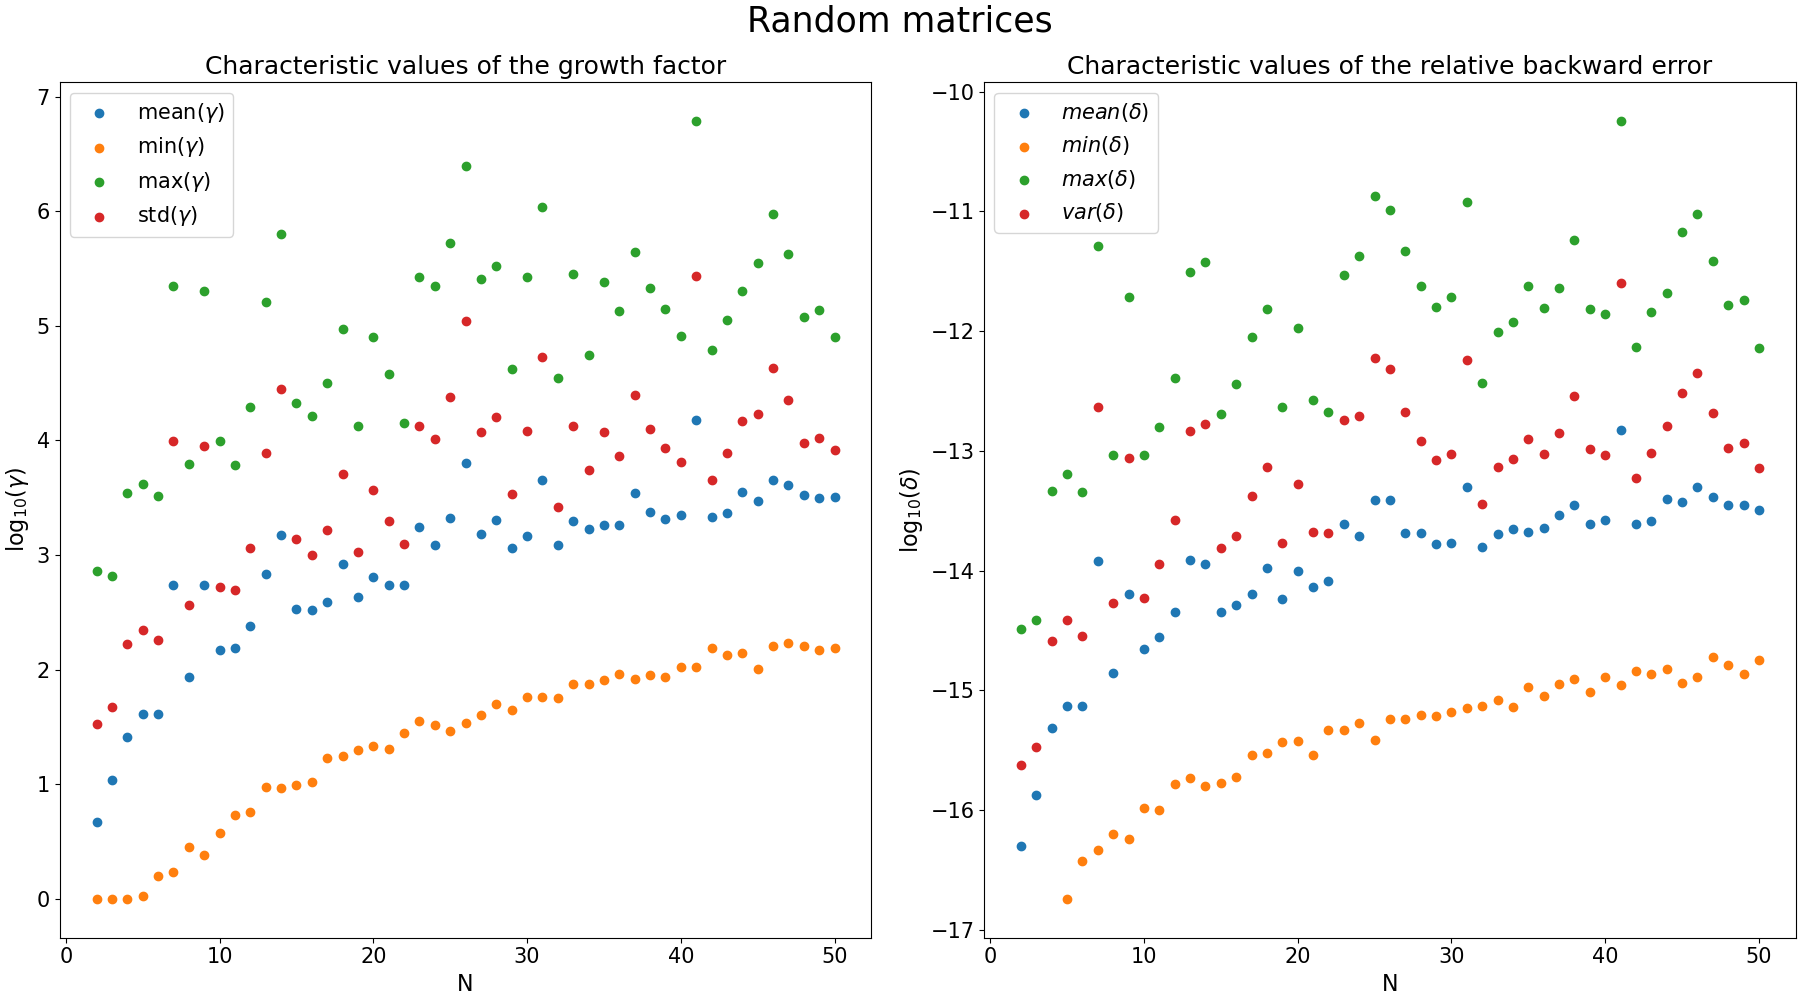
\includegraphics[scale=0.3]{C:/Users/cerra/Documents/GitHub/Numerical_Analysis_Optimization/Project_1_latex/Plot/Scatterplot_charact_values_for_Random_matrices}
	\caption{Scatterplot of the characteristic values of $\gamma$ and $\delta$ as a function of $N$ for real random matrices. Logarithmic scale on the ordinate axis.}
	\label{fig:Scatterplot_Random}
\end{figure}

\begin{figure}[H]
	\centering
	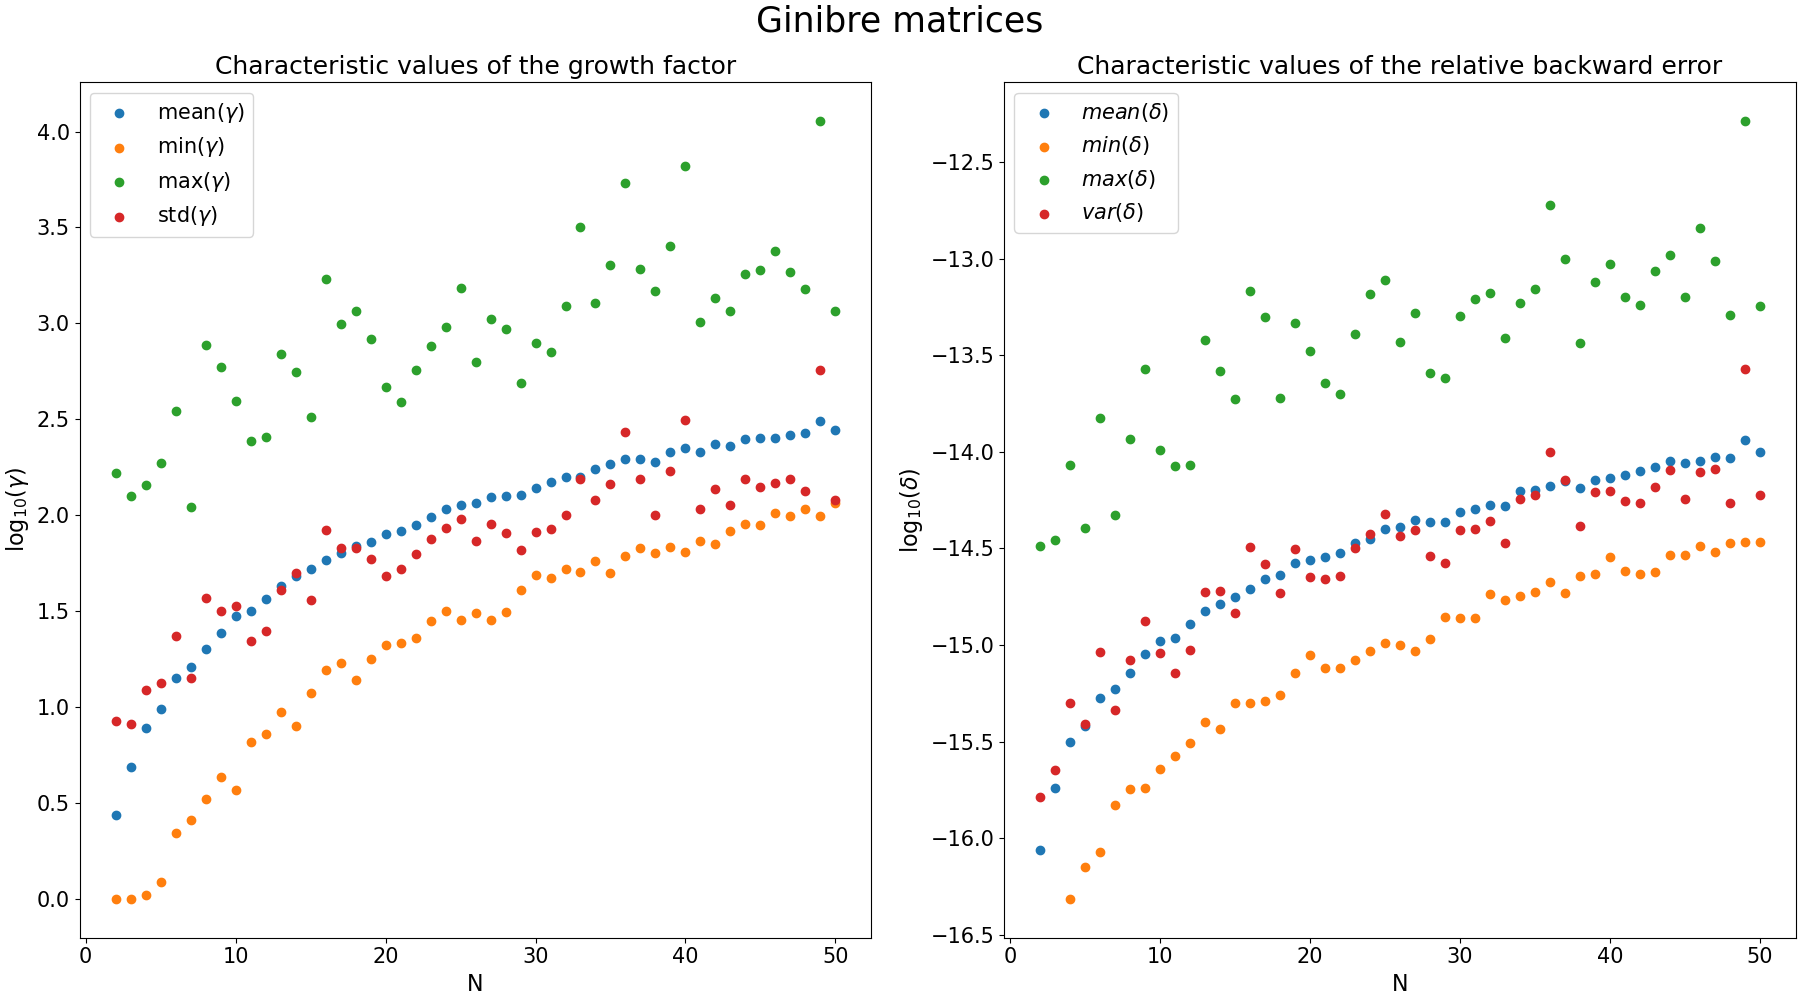
\includegraphics[scale=0.3]{C:/Users/cerra/Documents/GitHub/Numerical_Analysis_Optimization/Project_1_latex/Plot/Scatterplot_charact_values_for_Ginibre_matrices}
	\caption{Scatterplot of the characteristic values of $\gamma$ and $\delta$ as a function of $N$ for Ginibre matrices. Logarithmic scale on the ordinate axis.}
	\label{fig:Scatterplot_Ginibre}
\end{figure}
	
\noindent As can be seen from these plots, the characteristic values of the two considered quantities increase, as expected, with the dimension of the input matrix for both types of random matrices taken into account. This is due to the fact that, when the dimension of the input matrix increases, the algorithm that performs the LU factorization naturally requires more steps, resulting in an unavoidable propagation of numerical errors. It is interesting to also consider, for a fixed dimension, the distributions of the growth factor and the relative backward error for both cases. We have chosen to report here the histograms obtained for $N=25$, together with the corresponding boxplots, where the outliers have been removed for clarity of visualization. We have chosen this point as an intermediate representative dimension; similar considerations hold also in the other cases.
\begin{figure}[H]
	\centering
	\subfloat[][]{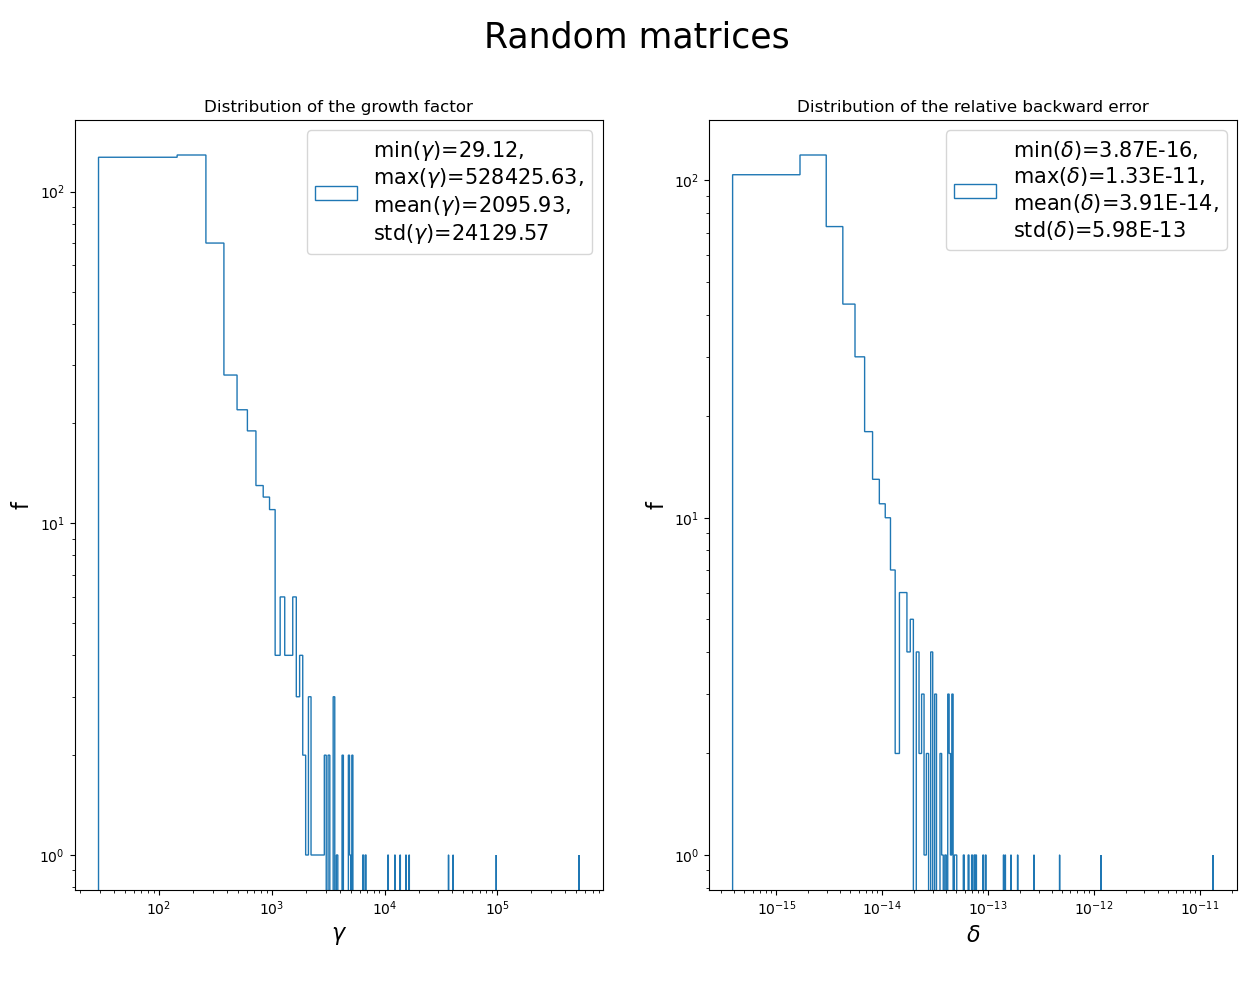
\includegraphics[scale=0.23]{C:/Users/cerra/Documents/GitHub/Numerical_Analysis_Optimization/Project_1_latex/Plot/Distributions_for_Random_matrices_of_dim_25}}\ \subfloat[][]{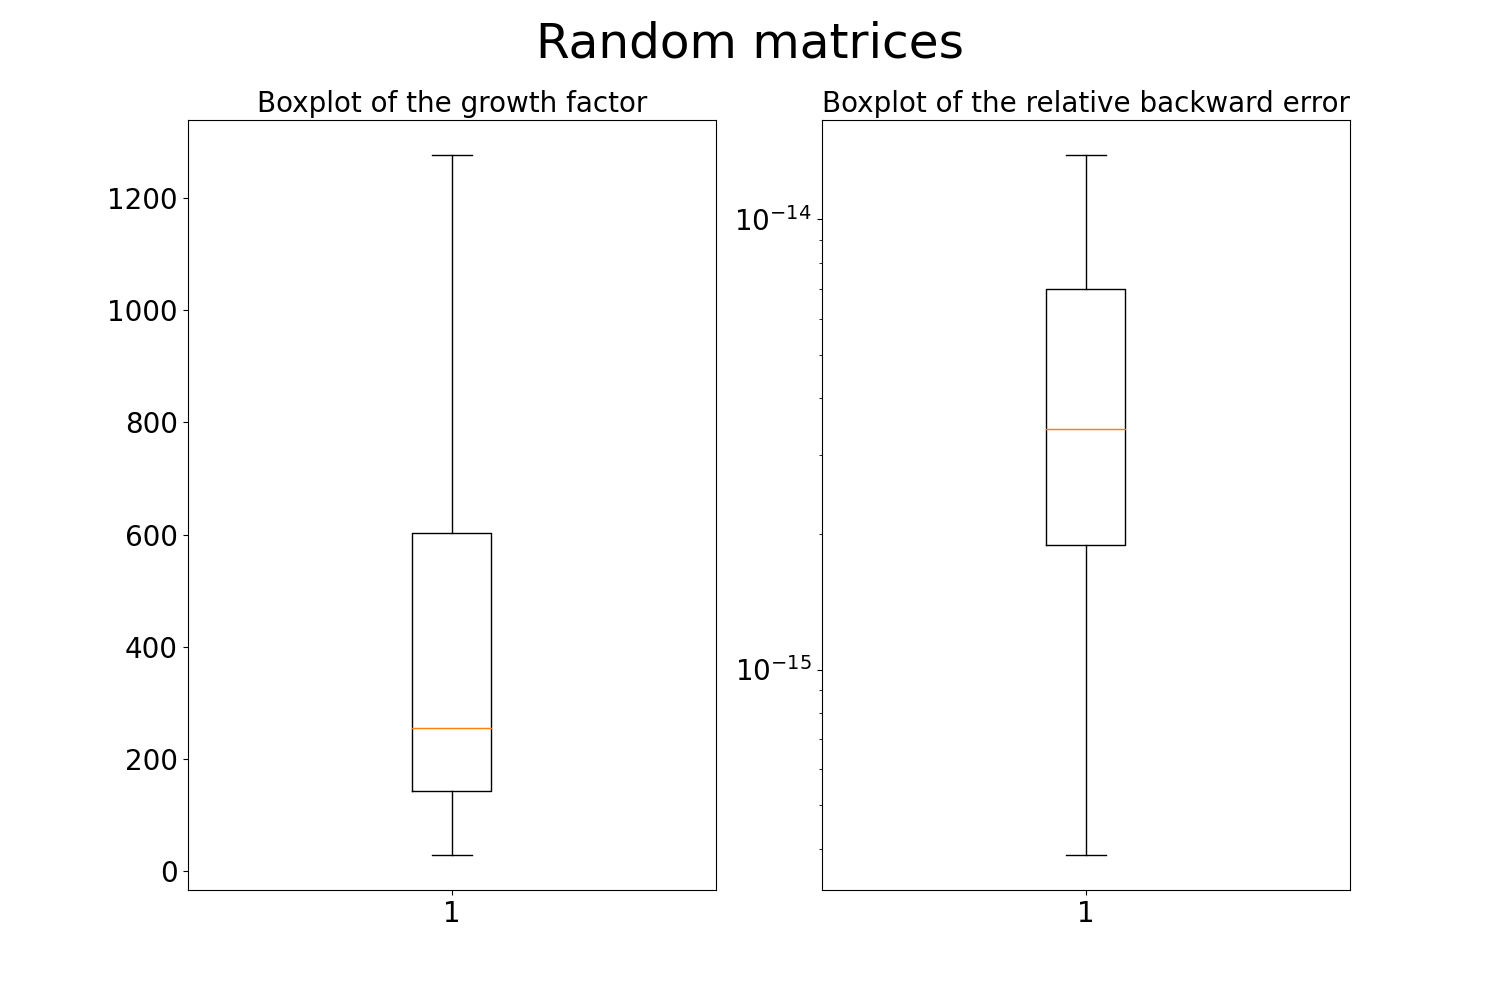
\includegraphics[scale=0.23]{C:/Users/cerra/Documents/GitHub/Numerical_Analysis_Optimization/Project_1_latex/Plot/Boxplot_for_Random_matrices_of_dim_25}}
	\caption{Histograms (panel (a)) and boxplots (panel (b)) of $\gamma$ and $\delta$ considering real random matrices of dimension $25\times 25$. Logarithmic scale are reported on both axis of the histograms as well as on the ordinate axes of the relative backward error boxplot.}
	\label{fig:Distributions and boxplot Random Matrices N=25}
\end{figure}

\begin{figure}[H]
	\centering
	\subfloat[][]{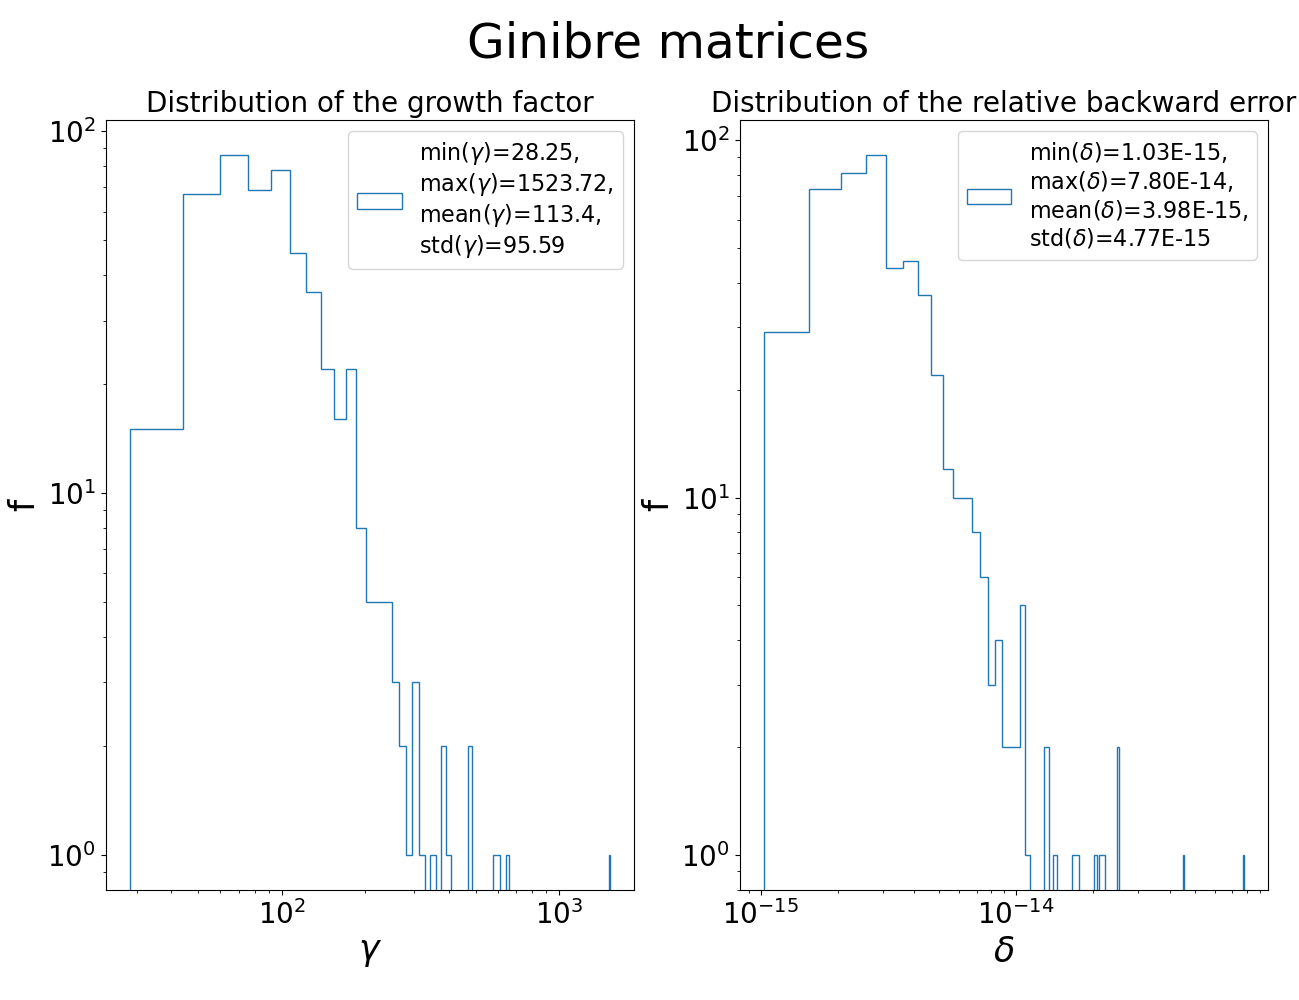
\includegraphics[scale=0.23]{C:/Users/cerra/Documents/GitHub/Numerical_Analysis_Optimization/Project_1_latex/Plot/Distributions_for_Ginibre_matrices_of_dim_25}}\ \subfloat[][]{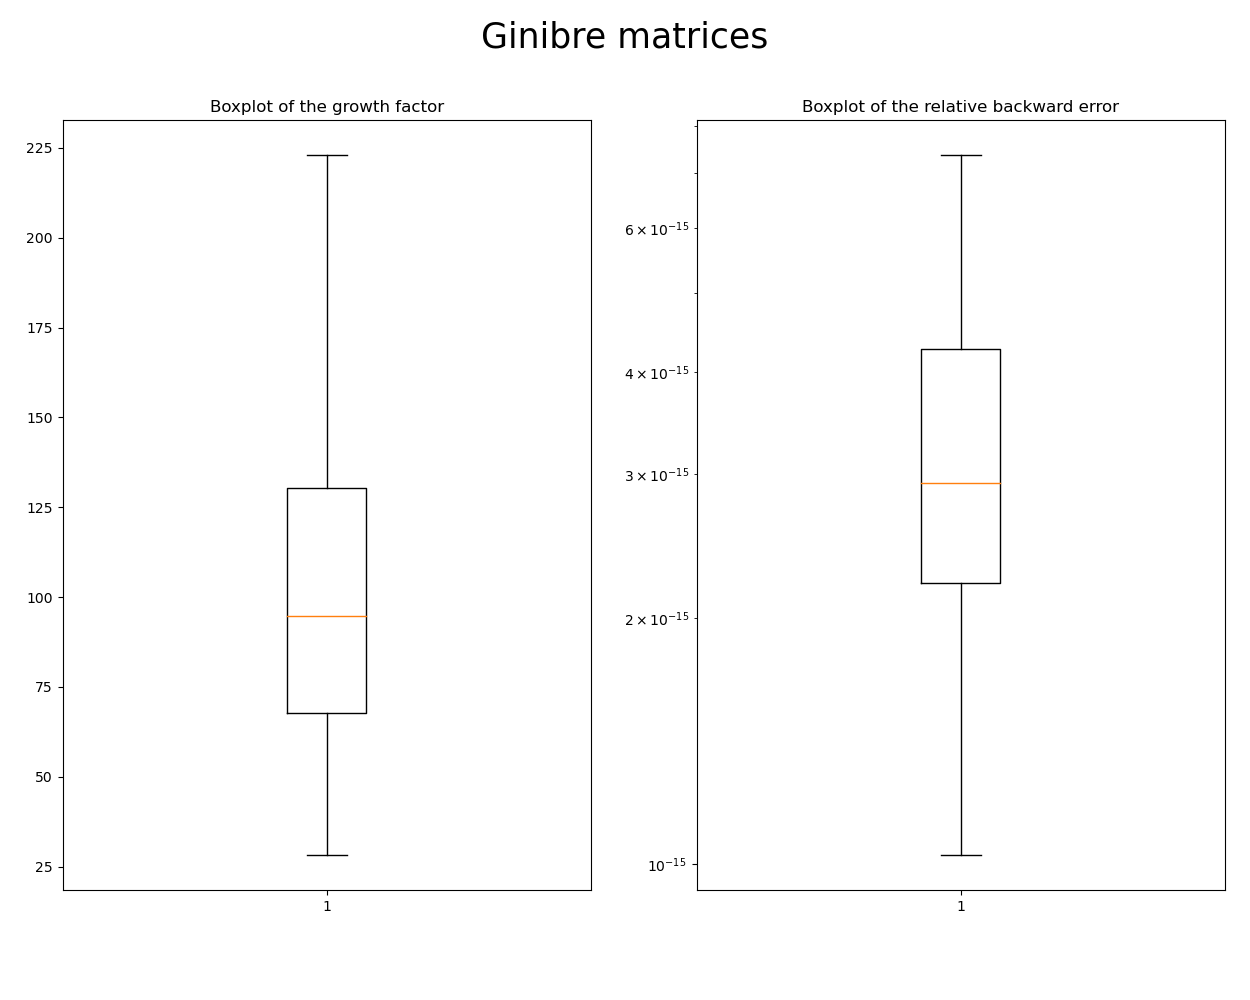
\includegraphics[scale=0.23]{C:/Users/cerra/Documents/GitHub/Numerical_Analysis_Optimization/Project_1_latex/Plot/Boxplot_for_Ginibre_matrices_of_dim_25}}
	\caption{Histograms (panel (a)) and boxplots (panel (b)) of $\gamma$ and $\delta$ considering Ginibre matrices of dimension $25\times 25$. Logarithmic scale are reported on both axis of the histograms as well as on the ordinate axes of the relative backward error boxplot.}
	\label{fig:Distributions and boxplot Ginibre Matrices N=25}
\end{figure}

\noindent It can be observed that both the growth factor and the relative backward error have a wider rage of variation, if one also consider outliers, in the case of real random matrices (for this reason we have considered a logarithmic scale on the axis), while these ranges are smaller in the case of Ginibre matrices. This is, in general, an indication of the fact that both values strongly depend on the input matrix (remember that we have done $500$ iterations), even if more careful considerations can be made to distinguish the two cases. In fact, taking into account, for example, the relative backward error and considering also the outliers, one can note that for real random matrices whose entries are uniformly distributed in $\left[0,1\right)$, this quantity ranges from a minimum value that is of order $10^{-16}$ to a maximum value of order $10^{-11}$. For what concern the Ginibre matrices, the same quantity ranges from a minimum value of order $10^{-15}$ to a maximum value that is approximatively of order $10^{-13}$. It is worth noting that the presence of outliers is more marked in the first case. However, if one discards the outliers, the range of variation of the relative backward error is approximatively the same in both cases. The differences that turn out in this comparison might be due to the fact that when considering the normal distribution to sample the entries of a random matrix, it is more likely to have matrix elements that are centred in the neighbourhood of the mean value, resulting in an ensemble of more homogeneous matrices. This, as a consequence, might reflect in relative backward errors, when computing the LU factorization of these matrices, that are similar and have a smaller range of variation. In the other case, when considering the uniform distribution to sample the entries of a random matrix, the resulting ensemble of matrices can be less homogeneous when compared to the previous one, and this might result in a wider range of variation of the quantity under examination. However, even if in both cases the relative backward errors grow with the dimension of the matrix, their values are small enough and, at least for the mean value, not that far from the machine epsilon, that is of order $10^{-16}$, so the algorithm can be considered backward stable for these types of random matrices.

\subsubsection*{Unitary matrices} We considered in out dataset the ensemble of unitary matrices, namely matrices $U$ such that $U^{*} = U^{-1}$, where $*$ stands for the conjugate transpose. These matrices have been sampled using the \mintinline{Python}{tenpy} Python library and they are also called \textit{CUE matrices}, as they are sampled from the circular ensemble. As in the previous case, we report in the following the scatterplot of the growth factor $\gamma$ and the relative backward error $\delta$ as a function of the dimension $N$ of the matrix.
%We know from theory that the eigenvalues of these matrices are the roots of the unity and, therefore, they all have absolute value equals to one (they are said to be unimodular). 
%For this reason, we expect the LU factorization algorithm to be backward stable
\begin{figure}[H]
	\centering
	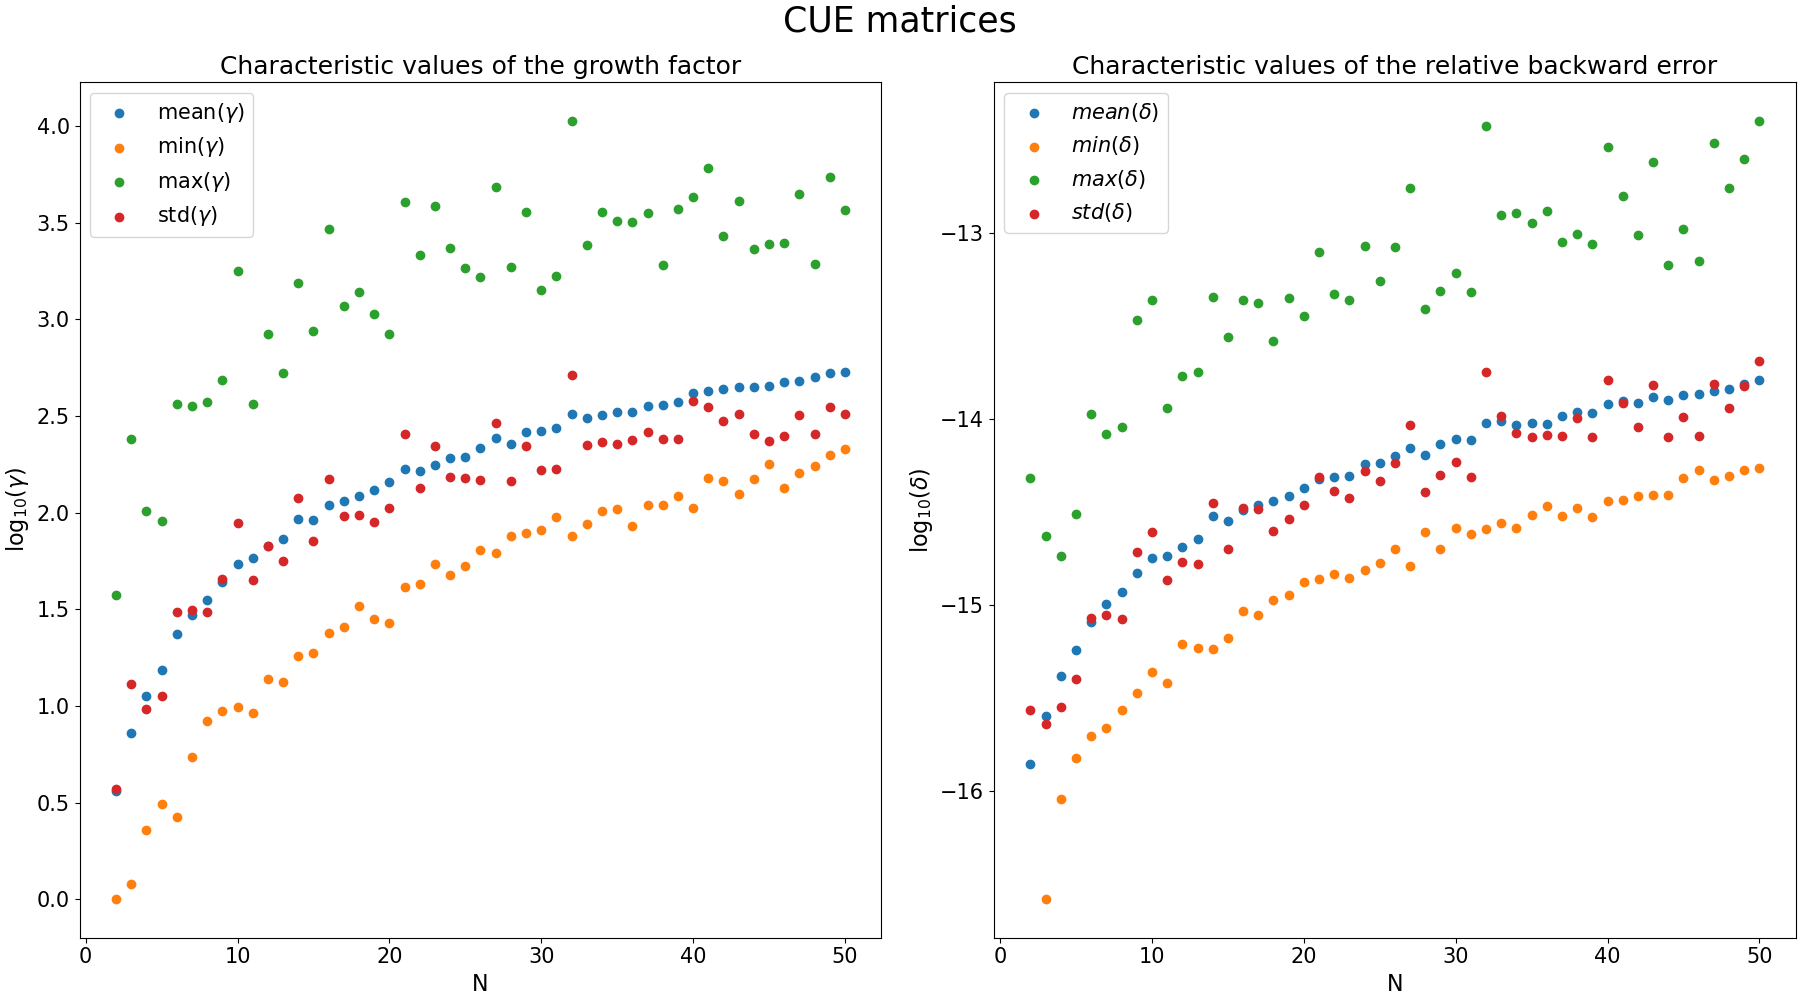
\includegraphics[scale=0.3]{C:/Users/cerra/Documents/GitHub/Numerical_Analysis_Optimization/Project_1_latex/Plot/Scatterplot_charact_values_for_CUE_matrices}
	\caption{Scatterplot of the characteristic values of $\gamma$ and $\delta$ as a function of $N$ for unitary matrices. Logarithmic scale on the ordinate axis.}
	\label{fig:Scatterplot_CUE}
\end{figure}
\noindent As can be seen from the values obtained for the growth factor and the relative backward error, the LU factorization algorithm is backward stable for unitary matrices. Note that the range of variation of both these values is comparable with the one obtained in the case of Ginibre matrices, and the same considerations regarding the distribution of these values hold when considering a fixed matrix dimension.\\
%
%It turns out that this case is quite similar to the case of Ginibre matrices for what concern the range of variation of the characteristic values of both the growth factor and the relative backward error.
%*** This might be understood if one investigates how these matrices are generated in the source code of the \mintinline{Python}{tenpy} library. It can be seen, in fact, that unitary matrices are generated starting from a Ginibre matrix $A$, so a complex matrix whose entries are independent normally distributed, and then performing a QR decomposition, so $A=QR$, where $Q$ is a unitary matrix and $R$ is an upper triangular matrix, and then giving as output a properly rescaled version of the $Q$ matrix. ***
%However, we expect the LU factorization to be backward stable for unitary matrices, and the values of $\gamma$ and $\delta$ that we obtain suggest that this is the case.
%Therefore, it can be concluded that the LU factorization algorithm is backward stable, as expected, for unitary matrices.

\noindent \textbf{Hermitian matrices }  The next class of matrices that we considered is that of Hermitian matrices, namely matrices $H$ such that $H = H^{*}$. In order to sample these matrices we used the \mintinline{Python}{tenpy} Python library. These matrices are also called \textit{GUE matrices} as they are sampled from the Gaussian unitary ensemble.

\begin{figure}[H]
	\centering
	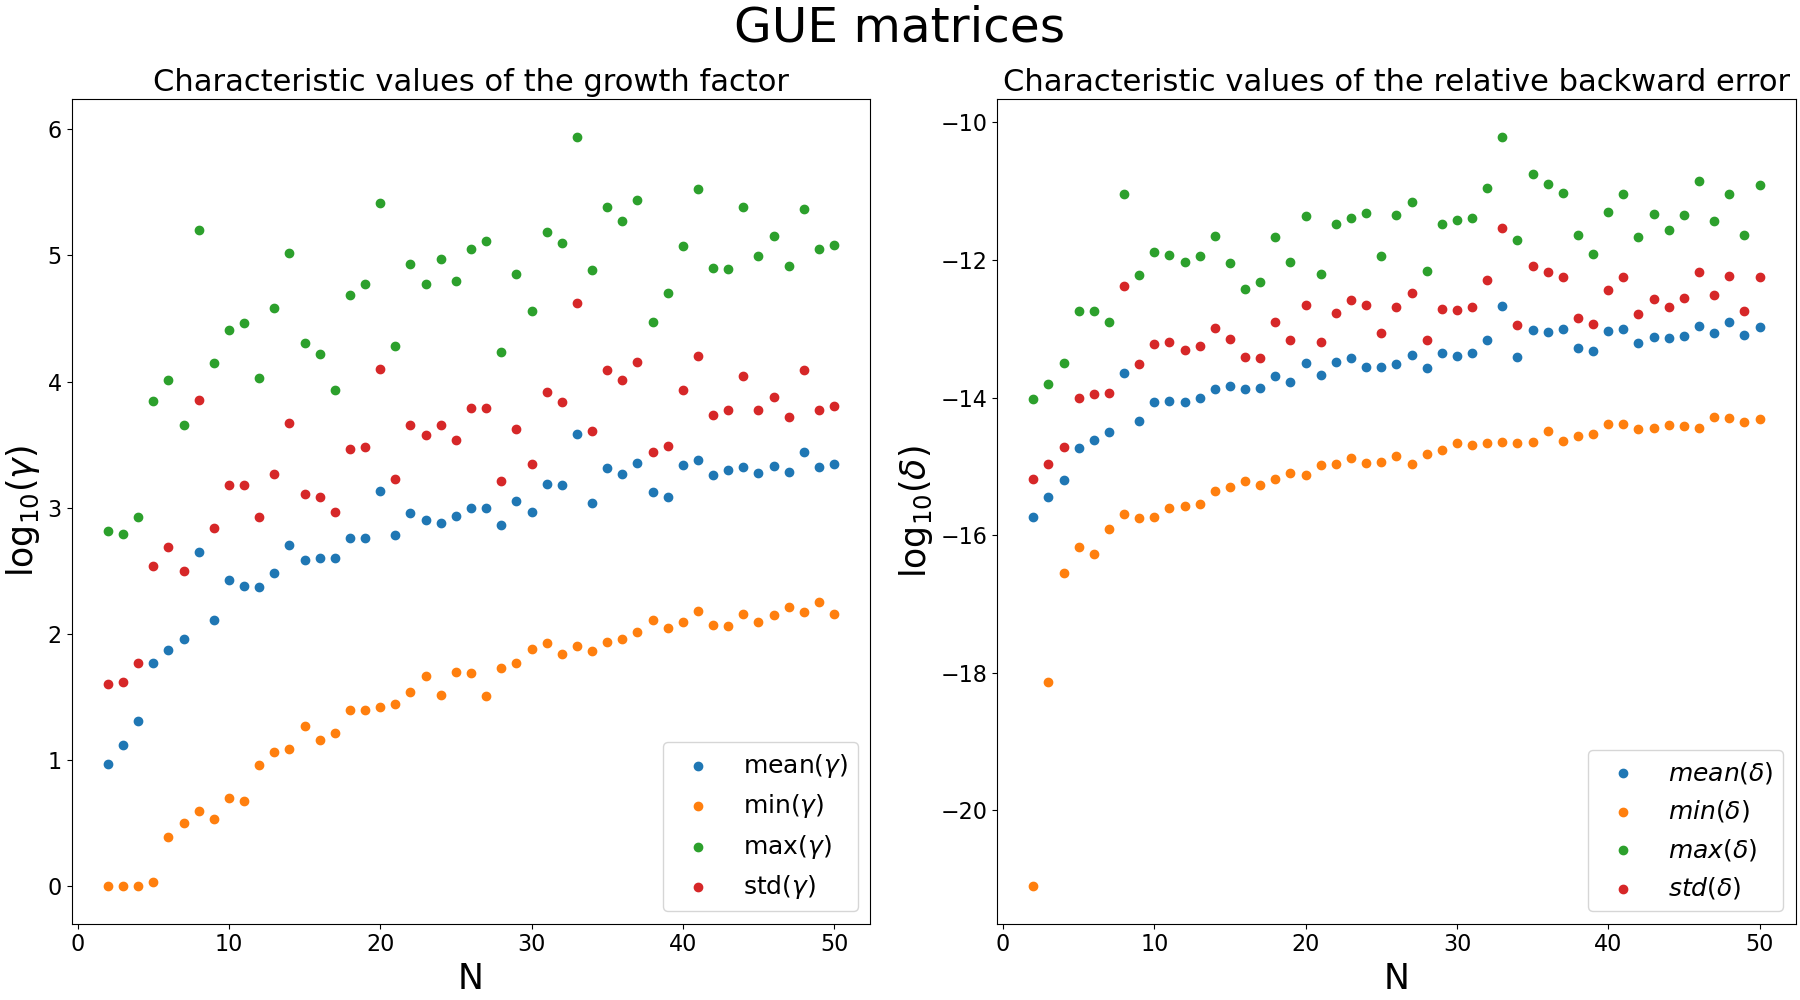
\includegraphics[scale=0.3]{C:/Users/cerra/Documents/GitHub/Numerical_Analysis_Optimization/Project_1_latex/Plot/Scatterplot_charact_values_for_GUE_matrices}
	\caption{Scatterplot of the characteristic values of $\gamma$ and $\delta$ as a function of $N$ for Hermitian matrices. Logarithmic scale on the ordinate axis.}
	\label{fig:Scatterplot_GUE}
\end{figure}

\noindent A common characteristic of all these scatterplots is that the range of variation of both the growth factor and the relative backward error is quite large, approximatively of two or three order of magnitude. The choice input matrix has, therefore, an impact in determining these values. However, as in the previous cases, these data suggest that the algorithm is backward stable for this class of matrices.\\

\noindent \textbf{Positive definite matrices } The penultimate class of matrices that we considered is that of positive definite matrices. Positive definite matrices $W$ can be obtained by considering matrices of the form $W = A^{*}A$, where $*$ stands for the conjugate transpose, discarding singular matrices. If the matrix $A$ is sampled from the Ginibre ensemble, that is it is a complex matrix whose entries are independent normally distributed, the matrix $W$ is called \textit{Wishart matrix}. In order to sample these matrices we used the \mintinline{Python}{qutip} Python library, considering, in particular, unit trace matrices. Note that matrices of this kind are also Hermitian. We expect the LU factorization for these matrices to be backward stable.\\

\noindent We report in the following the scatterplot of the growth factor and the relative backward error as a function of the dimension of the input matrix.

\begin{figure}[H]
	\centering
	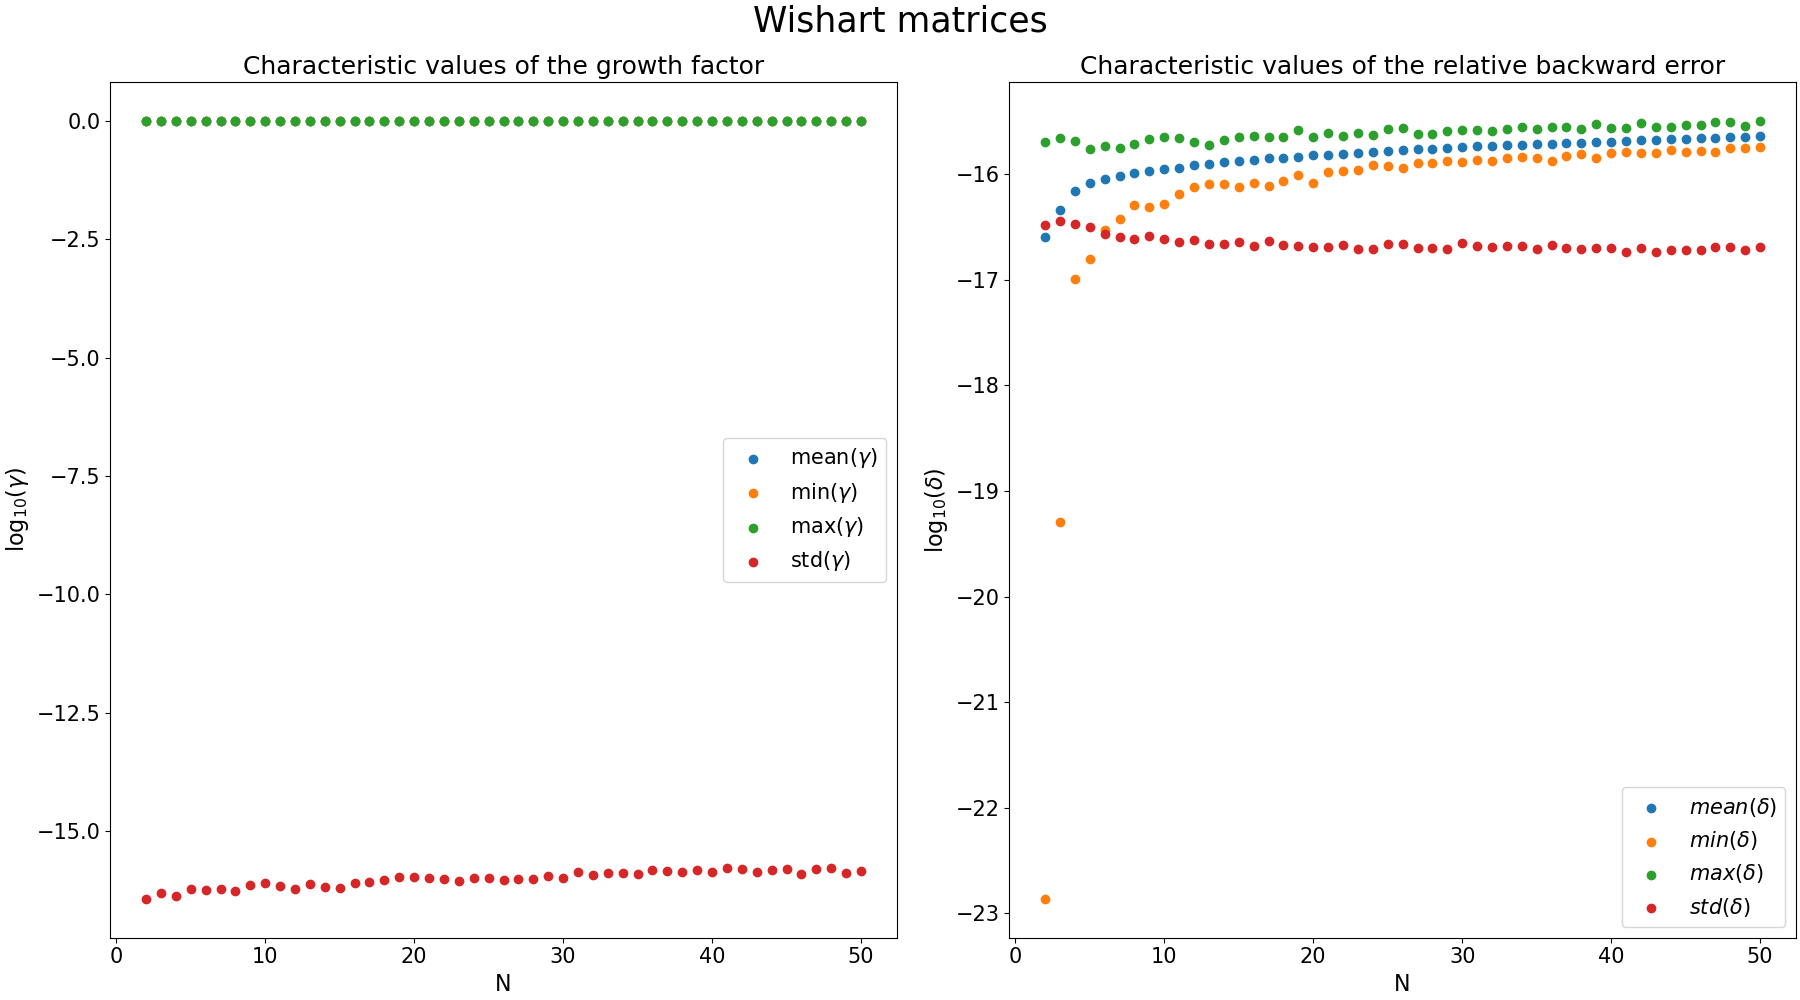
\includegraphics[scale=0.3]{C:/Users/cerra/Documents/GitHub/Numerical_Analysis_Optimization/Project_1_latex/Plot/Scatterplot_charact_values_for_Wishart_matrices}
	\caption{Scatterplot of the characteristic values of $\gamma$ and $\delta$ as a function of $N$ for positive definite matrices. Logarithmic scale on the ordinate axis.}
	\label{fig:Scatterplot_Wishart}
\end{figure}

\noindent It turns out that this case is quite different from the previous ones. In fact, it can be seen that the minimum, maximum and mean value of the growth factor are all equal to one, while the standard deviation is of the order of the machine epsilon. Moreover, the relative backward error is significantly small and it is of the order of the machine epsilon. It is interesting to note that, in this latter case, the standard deviation is smaller if compared to the other values, suggesting that the distribution of the relative backward error is peaked in correspondence with the mean value. This means that, differently from the other cases, whatever the input matrix, the values obtained for the backward error will be approximately the same or, in other words, they will be included in a very small range. This suggest a very strong backward stability of the LU factorization, as expected, for this class of matrices.\\

\noindent \textbf{Diagonally dominant matrices } The last class of matrices that we considered in our dataset is given by the diagonally dominant matrices. These are matrices whose diagonal entries are, in absolute value, greater or equal to the sum of the absolute values of the other elements in the corresponding row. We described how we sampled this matrices in the description of the dataset in the section ***** .\\
In the following we report the scatterplot of the growth factor and the relative backward error as a function of the dimension of the matrix.

\begin{figure}[H]
	\centering
	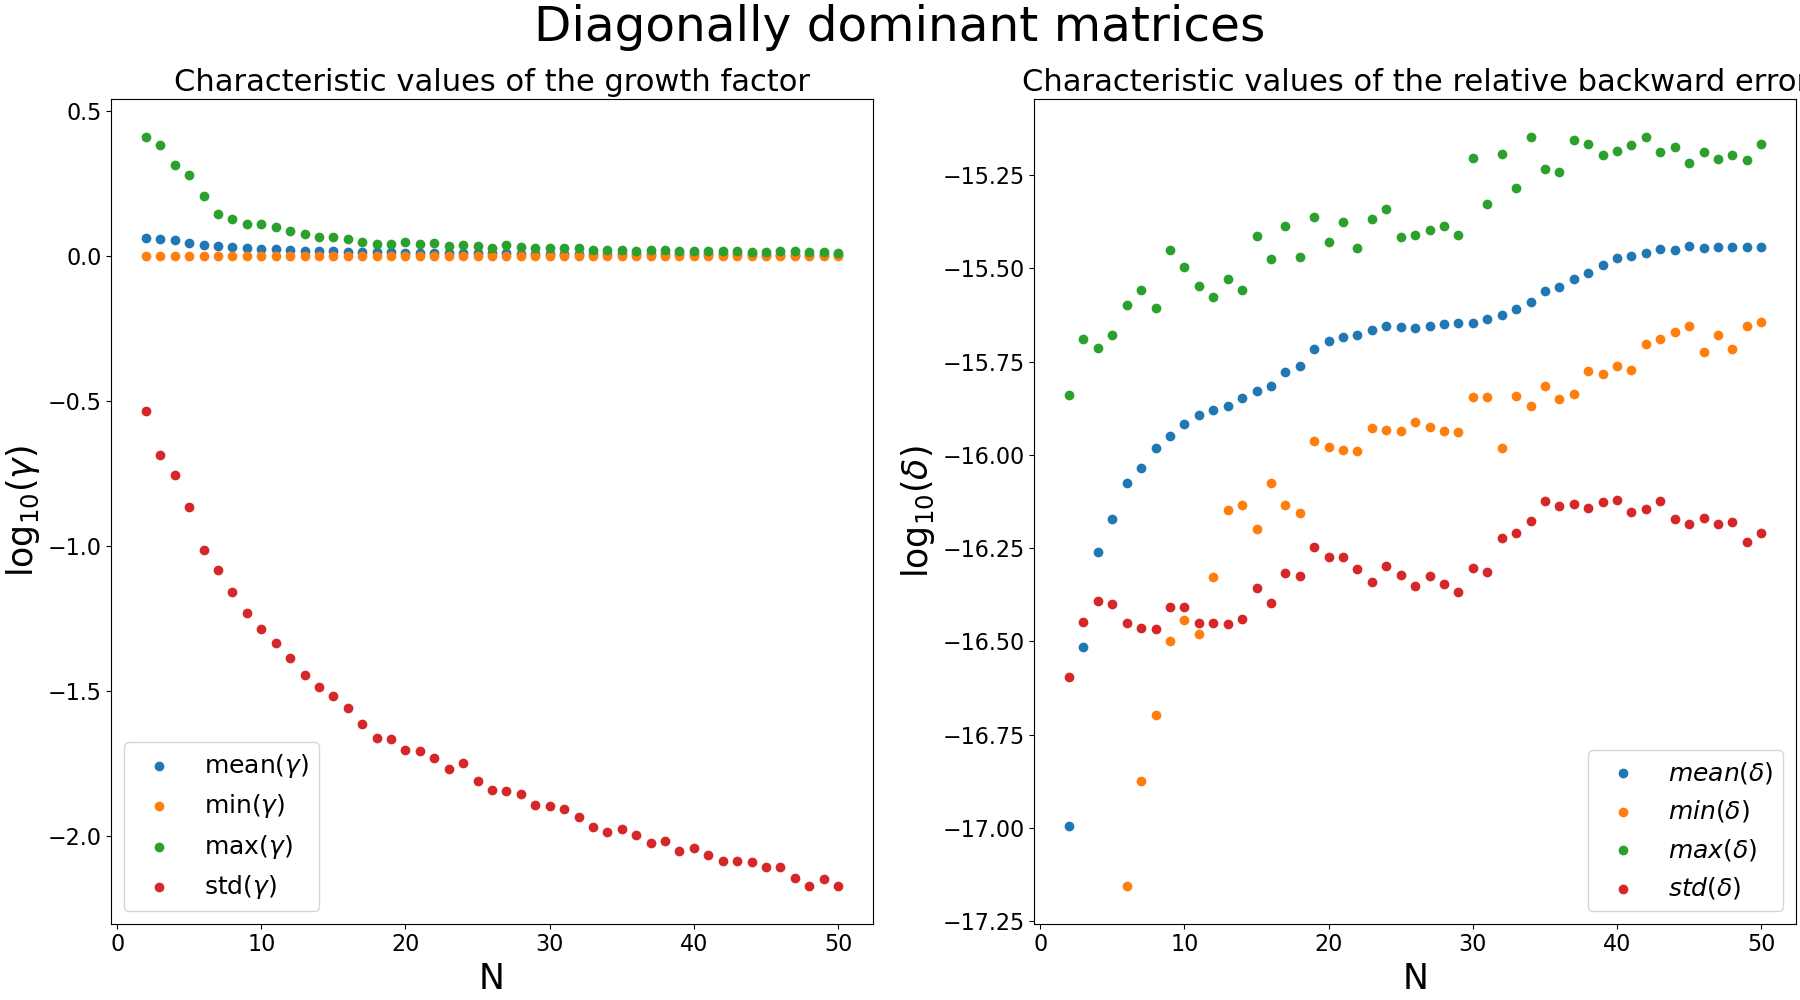
\includegraphics[scale=0.3]{C:/Users/cerra/Documents/GitHub/Numerical_Analysis_Optimization/Project_1_latex/Plot/Scatterplot_charact_values_for_Diagonally dominant_matrices}
	\caption{Scatterplot of the characteristic values of $\gamma$ and $\delta$ as a function of $N$ for diagonally dominant matrices. Logarithmic scale on the ordinate axis.}
	\label{fig:Scatterplot_Diag_dom}
\end{figure}

\noindent In this case, considerations similar to the case of positive definite matrices can be made. In fact, it can be observed that the growth factor is of order $\mathcal{O}(1)$, while the relative backward error is of the order of the machine epsilon, with the standard deviation that suggests, as in the previous case, that the distribution of this quantity, for a fixed dimension of the input matrix, is peaked at the mean value. Therefore, the value obtained for this quantity does not strongly depend on the input matrix. It can be concluded that the LU factorization is backward stable for this class of matrices.

\subsubsection{Conclusions}
Given the classes of matrices considered in the dataset, we found that the LU factorization is backward stable in all the cases considered, with differences that emerges when comparing the last two types of matrices considered, namely positive definite and diagonally dominant matrices, to the other ones. In fact, in these last two case, the LU factorization is strongly backward stable and the values obtained for what concern the relative backward error do not depend on the input matrix, differently from the other cases, where this happen. In the following we report a final plot where we compare the boxplots of all the types of matrices taken into account when considering a fixed dimension of the input matrix, that is $N=25$. Note that, for greater clarity of visualization, we discard outliers and consider, in this way, the most likely range of possible values.

\begin{figure}[H]
	\centering
	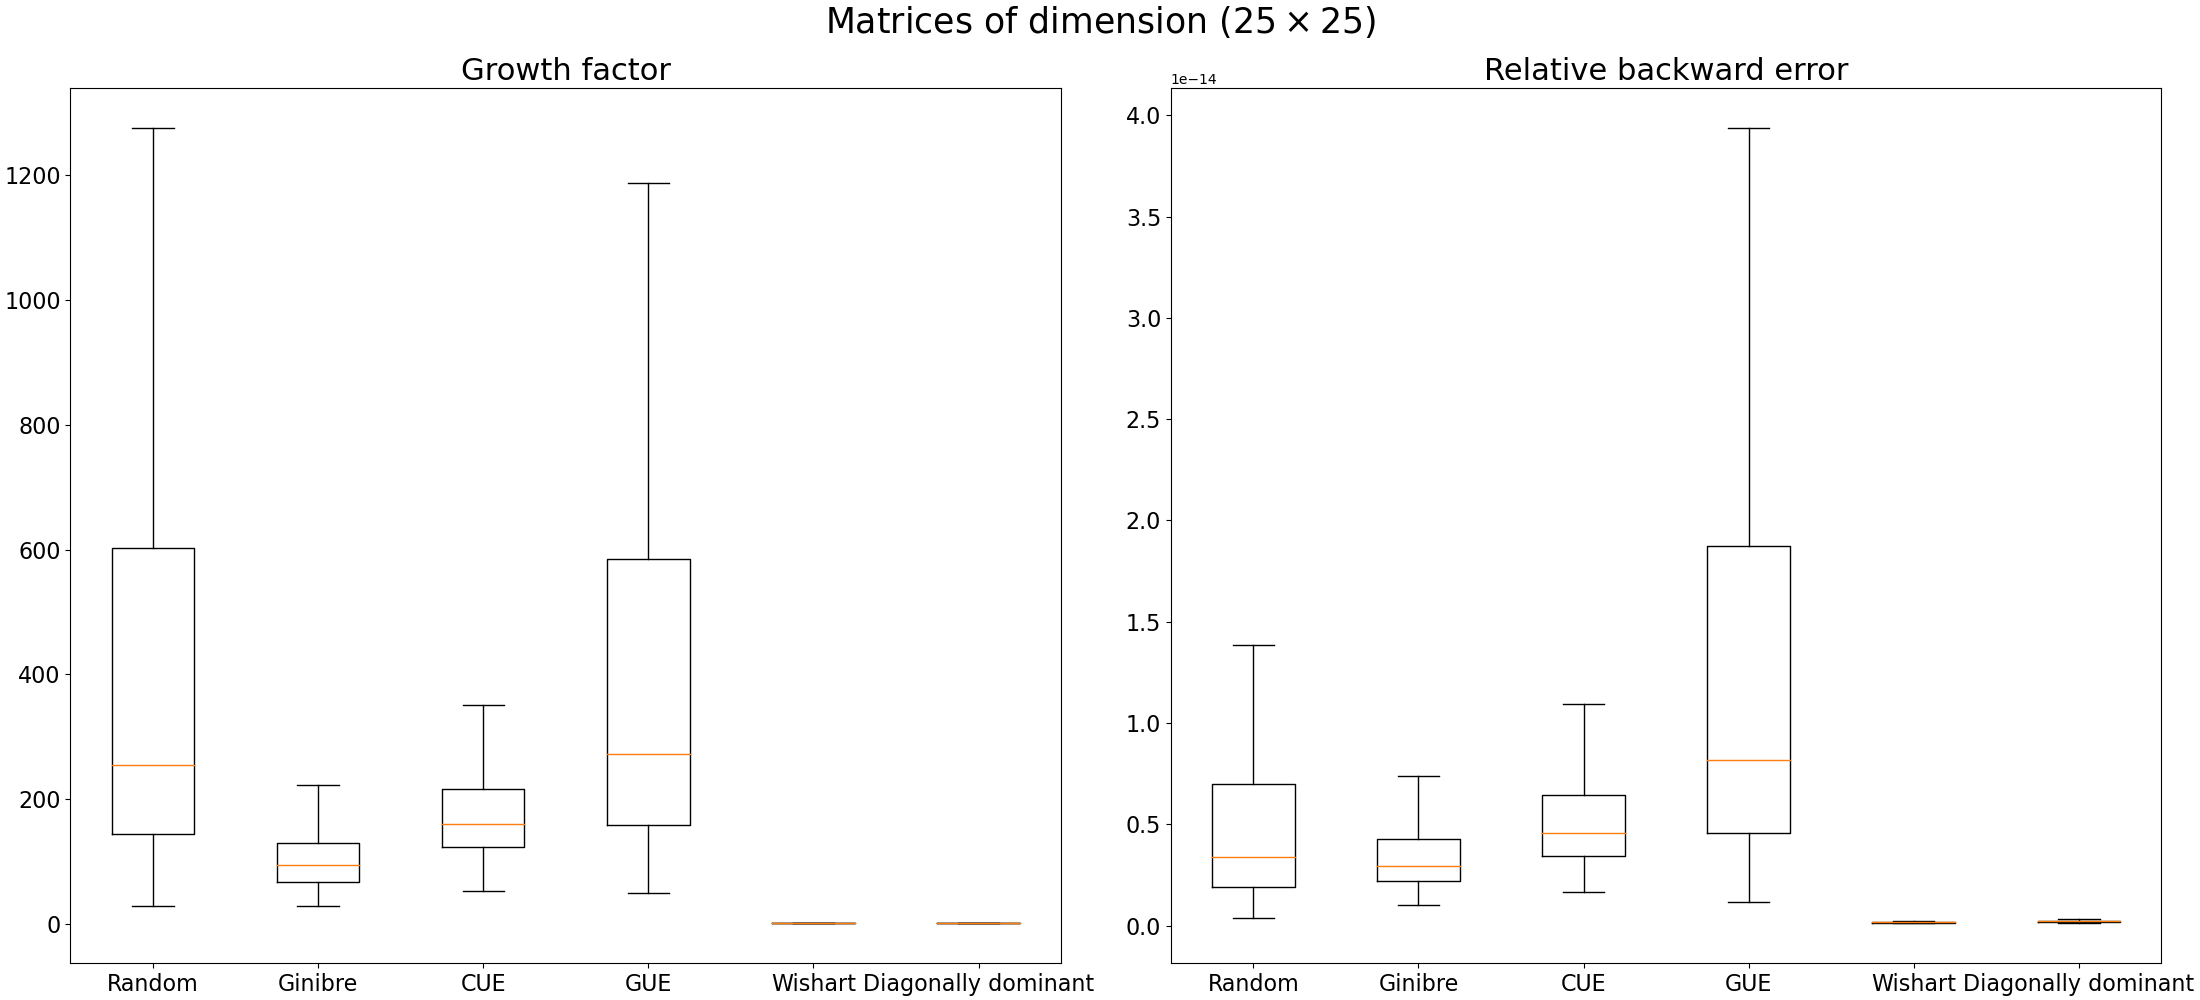
\includegraphics[scale=0.25]{C:/Users/cerra/Documents/GitHub/Numerical_Analysis_Optimization/Project_1_latex/Plot/Boxplot_dim_matr=25}
	\caption{Boxplot of $\gamma$ and $\delta$ for matrices of dimension $25\times25$.}
	\label{fig:Boxplot_final}
\end{figure}

\newpage
	Hilbert matrices becomes numerically singular starting from $N=6$, but the LU factorization is still possible (maybe).
	The LU factorization breaks down for $N=21$ (if one compares the absolute value of the element $A_{kk}$ at the step $k-1$, namely $A_{kk}^{k-1}$, with the machine precision), while it breaks down for $N=15$ if one compares the same two values without considering the absolute value for the first one. What does it mean for us that the LU factorization breaks down? We are comparing the element $A_{kk}^{k-1}$ with the machine precision but maybe this is not the best strategy possible as the relative backward error is still zero, even for larger $N$ values. This is probably due to the fact that such numbers can still be represented in the computer. In fact, the algorithm gives us the correct (maybe) matrices $L$ and $U$ such that $A=LU$f(k).
	
	
	
	
\end{document}